% !TeX program = xelatex
% !TeX encoding = UTF-8
% !TeX spellcheck = en_US
% !BIB program = biber
%% 
%% The above lines help editors like TeXstudio to automatically choose the right tools
%% to compile your LaTeX source file. If your tool does not support these magic comments,
%% you will need to make appropriate manual choices.
%% 
%% You can safely use "pdflatex" instead of "xelatex" if you prefer the pdfLaTeX toolchain.
%% However, pdfLaTeX will not be able to deliver the professional font experience that you
%% will get with XeLaTeX. You can also safely use "lualatex" instead of "xelatex" while
%% preserving the professional font experience if you prefer the LuaLaTeX toolchain.
%% 
%% _Important_: These magic comments should be on the first lines of your source file.
%% 
%%%%%%%%%%%%%%%%%%%%%%%%%%%%%%%%%%%%%%%%%%%%%%%%%%%%%%%%%%%%%%%%%%%%%%%%%%%%%%%%

%%%%%%%%%%%%%%%%%%%%%%%%%%%%%%%%%%%%%%%%%%%%%%%%%%%%%%%%%%%%%%%%%%%%%%%%%%%%%%%%
%% 
%%            JJJJ   K                         K   UUUU         UUUU  
%%            JJJJ   KKKK                   KKKK   UUUU         UUUU  
%%            JJJJ   KKKKKK               KKKKKK   UUUU         UUUU  
%%            JJJJ      KKKKKK         KKKKKK      UUUU         UUUU  
%%            JJJJ         KKKKKK   KKKKKK         UUUU         UUUU  
%%            JJJJ            KKKKKKKKK            UUUU         UUUU  
%%    JJ     JJJJJ               KKK               UUUUU       UUUUU  
%%  JJJJJJJJJJJJJ    KKKKKKKKKKKKKKKKKKKKKKKKKKK    UUUUUUUUUUUUUUU   
%%    JJJJJJJJJ      KKKKKKKKKKKKKKKKKKKKKKKKKKK      UUUUUUUUUUU     
%% 
%% This is an example file for using the JKU LaTeX technical report template
%% for your technical report.
%% 
%% Template created by Michael Roland (2021)
%% 
%%%%%%%%%%%%%%%%%%%%%%%%%%%%%%%%%%%%%%%%%%%%%%%%%%%%%%%%%%%%%%%%%%%%%%%%%%%%%%%%

%%%%%%%%%%%%%%%%%%%%%%%%%%%%%%%%%%%%%%%%%%%%%%%%%%%%%%%%%%%%%%%%%%%%%%%%%%%%%%%%
%% 
%% Document class: This is a koma-script article.
%% 
\documentclass[a4paper,oneside,10pt,ngerman,english]{scrartcl}
%% 
%% The comma-separated list in square brackets are class options.
%% Useful options that you might want to use:
%% 
%% Paper size:
%%  * a4paper ... A4 paper size
%% 
%% Optimize for single-sided or double-sided printing:
%%  * oneside ... single-sided
%%  * twoside ... double-sided
%% 
%% Base font size:
%%  * 10pt ... 10-pt font is used for normal text
%%  * 11pt ... 11-pt font is used for normal text
%% 
%% Define document languages (the last specified language becomes the document default
%% language):
%%  * ngerman ... German
%%  * english ... English
%%  * ...
%% 
%% Alternate document classes: The JKU report template supports the koma-script classes
%% `scrartcl', `scrreprt' and `scrbook'. The article class `scrartcl' is well-suited
%% for a typical technical report. However, `scrbook' or `scrreprt' may be better
%% suited for longer reports since they permit structuring your work in chapters.
%%  
%% _Important_: The document class should be the first line of LaTeX code in your main
%% source file. Do not place anything but comments / magic comments above that line (unless
%% you really know what you are doing).
%% 
%%%%%%%%%%%%%%%%%%%%%%%%%%%%%%%%%%%%%%%%%%%%%%%%%%%%%%%%%%%%%%%%%%%%%%%%%%%%%%%%

%%%%%%%%%%%%%%%%%%%%%%%%%%%%%%%%%%%%%%%%%%%%%%%%%%%%%%%%%%%%%%%%%%%%%%%%%%%%%%%%
%% 
%% Treat input files as UTF-8 encoded. Make sure to always load this when you use pdfLaTeX
%% so that pdfLaTeX knows how to read and interpret characters in this source file.
%% 
\usepackage[utf8]{inputenc}
%% 
%%%%%%%%%%%%%%%%%%%%%%%%%%%%%%%%%%%%%%%%%%%%%%%%%%%%%%%%%%%%%%%%%%%%%%%%%%%%%%%%

%%%%%%%%%%%%%%%%%%%%%%%%%%%%%%%%%%%%%%%%%%%%%%%%%%%%%%%%%%%%%%%%%%%%%%%%%%%%%%%%
%% 
%% Use the JKU LaTeX technical report template for this document.
%% 
\usepackage[techreport,fancyfonts,noautopdfinfo]{jkureport}
%% 
%% The comma-separated list in square brackets are theme options. Useful options that you
%% might want to use:
%% 
%% Document type:
%%  * phdthesis     ... PhD thesis.
%%  * mathesis      ... Master's thesis.
%%  * diplomathesis ... Diploma thesis.
%%  * bathesis      ... Bachelor's thesis.
%%  * seminarreport ... Seminar report.
%%  * techreport    ... Technical report.
%% 
%% Color scheme selection options:
%%  * JKU  ... Use JKU (gray) color scheme (this is the default if no scheme is selected).
%%  * BUS  ... Use Business School color scheme.
%%  * LIT  ... Use Linz Institute of Technology color scheme.
%%  * MED  ... Use MED faculty color scheme.
%%  * RE   ... Use RE faculty color scheme.
%%  * SOE  ... Use School of Education color scheme.
%%  * SOWI ... Use SOWI faculty color scheme.
%%  * TNF  ... Use TNF faculty color scheme.
%% 
%% Space-efficient monospace font options (requires XeTeX/LuaTeX):
%%  * compactmono   ... Use condensed fixed-width font everywhere.
%%  * nocompactverb ... Do not use condensed fixed-width font for verbatim and listings.
%% 
%% Style-breaking options:
%%  * noimprint      ... Do not insert imprint on title pages.
%%  * nojkulogo      ... Do not insert JKU & K logos on title pages.
%%  * capstitle      ... Set document title in capital letters.
%%  * nofancyfonts   ... Do not use custom TTF fonts with XeTeX/LuaTeX / supress pdfLaTeX warning.
%%  * equalmargins   ... Decrease the outer page margin to have both page margins of equal size
%%                       (the additional outer margin is intentional and to be used for
%%                       anotations; equalmargins also causes the text width to be
%%                       significantly larger than optimal for reading).
%% 
%% Experimental options:
%%  * mathastext ... Use standard document fonts (enhanced with symbols from Fira Math font
%%                   when using XeTeX/LuaTeX) in math mode.
%% 
%% Advanced options:
%%  * noautopdfinfo     ... Do not automatically try to add pdfinfo with hyperref from document
%%                          metadata fields.
%%  * logopath={<path>} ... Set the path where the theme can find its own logo resources. This
%%                          should typically be a relative path and the default is `./logos'.
%%  * fontpath={<path>} ... Set the path where the theme can find its own font resources. This
%%                          should typically be a relative path and the default is `./fonts'.
%% 
%% Hint: Boolean options can be used in the forms `option' or `option=true' the enable the
%% option and `nooption' or `option=false' to disable the option.
%% 
%%%%%%%%%%%%%%%%%%%%%%%%%%%%%%%%%%%%%%%%%%%%%%%%%%%%%%%%%%%%%%%%%%%%%%%%%%%%%%%%

%%%%%%%%%%%%%%%%%%%%%%%%%%%%%%%%%%%%%%%%%%%%%%%%%%%%%%%%%%%%%%%%%%%%%%%%%%%%%%%%
%% 
%% This is the place where you can load additional packages. If you want to load
%% a package `biblatex', you would use the command `\usepackage{biblatex}'.
%% 

\usepackage{csquotes}
\usepackage[backend=biber,citestyle=numeric,sortcites=true,maxcitenames=2,style=ACM-Reference-Format]{biblatex}
\setcounter{biburlnumpenalty}{100} %% reducing biburl* penalties typically improves URL placement in bibliography
\setcounter{biburllcpenalty}{100}
\setcounter{biburlucpenalty}{100}
\usepackage{todonotes}
\usepackage{import}
\usepackage{amsfonts}
\usepackage{subcaption}
\usepackage{float}
\usepackage{tikz}
\usetikzlibrary{fit,shapes,arrows,positioning}
%\usepackage{acronym}

%% 
%%%%%%%%%%%%%%%%%%%%%%%%%%%%%%%%%%%%%%%%%%%%%%%%%%%%%%%%%%%%%%%%%%%%%%%%%%%%%%%%

%%%%%%%%%%%%%%%%%%%%%%%%%%%%%%%%%%%%%%%%%%%%%%%%%%%%%%%%%%%%%%%%%%%%%%%%%%%%%%%%
%% 
%% Bibliography data files.
%% 

\addbibresource{references.bib}

%% 
%%%%%%%%%%%%%%%%%%%%%%%%%%%%%%%%%%%%%%%%%%%%%%%%%%%%%%%%%%%%%%%%%%%%%%%%%%%%%%%%

\begin{document}
%%%%%%%%%%%%%%%%%%%%%%%%%%%%%%%%%%%%%%%%%%%%%%%%%%%%%%%%%%%%%%%%%%%%%%%%%%%%%%%%
%% 
%% Report information and title page
%% 

%% Command \title{title}: sets the title of your report
\title{Analysis of Power Consumption of Home and SME Network Devices}

%% Command \titleshort{short title}: sets an abbreviated version of the report title for page heads
%\titleshort{Optional space for your abbreviated title}

%% Command \subtitle{subtitle}: sets the subtitle for seminar/technical reports (not used for theses)
\subtitle{Technical Report\\%
    \usekomafont{subtitlesmall}%
    \hfill\\%
    Master Project about the Analysis of Power Consumption of different Home and SME Network Equipment.
    \hfill\\%
}

%% Command \author{name}: sets the author name(s); separate multiple authors with \and; use \prefix{}
%%   and \suffix{} to add academic titles and suffixes (if needed); use \affiliation{} to add an
%%   affiliation, use \authornewline to add line breaks (e.g. to separate authors from contact
%%   information), use \authormail{}, \authorweb{}, \authorphone{} and \authorfax{} to add contact
%%   information)
\author{%
    Michael Reinegger
    \affiliation{Institute of Networks~and~Security}
    \authornewline
    \authormail{k12102754@students.jku.at}
    \authornewline
}

%% Command \date{YYYY-MM-DD}: set the day of publication (defaults to today)
%\date{2020-04-09}

%% Command \partnerlogo{filename}: use filename as partnerlogo, filename may be blank to disable the logo
%\partnerlogo{logos/ins}

%% Command \revisionblock{text}: set the document revision block on the title page
\revisionblock{V0.1 Initial Topic definition + Research Questions + Initial Test Setup and potential future Setup Ideas}

%% Command \reportnumber{number}: set the report number
%\reportnumber{Space for your report number}

%% Command \setbottommark{text}: set the bottom mark (in document footer)
%\setbottommark{Space for your bottom mark}

%% Command \abstract{text}: set the document abstract on the title page
%%\abstract{Space for your (short) abstract.}

%% Command \keywords{text}: set the document keywords
%\keywords{Space for your comma-separated keywords}


%% Finally, print the title page using the above information:
\maketitle
%% 
%%%%%%%%%%%%%%%%%%%%%%%%%%%%%%%%%%%%%%%%%%%%%%%%%%%%%%%%%%%%%%%%%%%%%%%%%%%%%%%%

%%%%%%%%%%%%%%%%%%%%%%%%%%%%%%%%%%%%%%%%%%%%%%%%%%%%%%%%%%%%%%%%%%%%%%%%%%%%%%%%
%% 
%% Add a table of contents
%% 

%% Make sure to start the table of contents on a new odd page (odd is only relevant in twoside layout)
\cleardoubleoddpage
%% Print the table of contents
\tableofcontents

%% Make sure to start the list of acronyms on a new odd page (odd is only relevant in twoside layout)
%\cleardoubleoddpage
%% Include list of acronyms (optional and often not necessary)
%\import{./}{acronyms}

%% 
%%%%%%%%%%%%%%%%%%%%%%%%%%%%%%%%%%%%%%%%%%%%%%%%%%%%%%%%%%%%%%%%%%%%%%%%%%%%%%%%

%%%%%%%%%%%%%%%%%%%%%%%%%%%%%%%%%%%%%%%%%%%%%%%%%%%%%%%%%%%%%%%%%%%%%%%%%%%%%%%%
%% 
%% Abstract: Instead of an abstract on the title page (see \abstract{...}), you
%% sometimes want to add an abstract as its own unnumbered section.
%% 

%% (Optionally) let the abstract start on a new odd page (odd is only relevant in twoside layout)
\cleardoubleoddpage

\addsec{Abstract}
This project provides a comprehensive analysis of the power consumption of network devices in home and Small and Medium-sized Enterprise (SME) environments. We investigate how factors such as network load, the number of connected clients, and connection types (Ethernet vs. Wi-Fi) influence energy usage. Using a dedicated testbed with automated data collection, we evaluate the real-world power efficiency of various consumer-grade, ISP-provided, and business-grade devices. The findings can lead to reducing energy consumption with more energy-efficient network devices and configurations.

%% 
%%%%%%%%%%%%%%%%%%%%%%%%%%%%%%%%%%%%%%%%%%%%%%%%%%%%%%%%%%%%%%%%%%%%%%%%%%%%%%%%

%%%%%%%%%%%%%%%%%%%%%%%%%%%%%%%%%%%%%%%%%%%%%%%%%%%%%%%%%%%%%%%%%%%%%%%%%%%%%%%%
%% 
%% Add your report sections ...
%% 

%% (Optionally) let the main sections start on a new odd page (odd is only relevant in twoside layout)
\cleardoubleoddpage

\section{Introduction}
\label{sec:introduction}

This project aims to analyze the power consumption of various network devices commonly used in home and small-to-medium enterprise (SME) environments. The equipment under investigation ranges from consumer-grade home routers to ISP-provided devices and business-grade switches and access points. The goal is to create a comprehensive overview of power consumption across different scenarios and usage patterns.

The analysis will examine several factors that influence power consumption: the number of active Ethernet ports, the number of connected Wi-Fi clients, varying levels of network load and so on. Data will be collected using a smart power meter capable of providing time-based power consumption measurements. This meter is integrated with a monitoring stack (Prometheus and Grafana) to enable automated data collection and visualization.

With this data, we can evaluate the efficiency of these devices under different conditions and identify which configurations are most power-efficient for specific use cases. For example, we can compare whether using an ISP-provided router in bridge mode is more efficient than using a separate router and switch/modem combination. Additionally, the analysis will help determine if some devices should be powered down during periods of low activity, such as overnight, to conserve energy.


\section{Research Questions}
\label{sec:research-questions}
\begin{itemize}
    \item How does power consumption change with the number of active Ethernet ports? Is there a measurable difference between 100 Mbps and 1 Gbps connections, in different load scenarios?
    \item How does power consumption scale with network load (idle, 50\%, 100\% utilization of bandwidth)?
    \item Which equipment is suitable for continuous operation and which devices have high idle consumption that makes them candidates for automated shutdown during off-peak hours?
    \item How does power consumption per client differ between Ethernet and Wi-Fi connections? Is there a threshold where Wi-Fi becomes more efficient on a per-client basis?
    \item What is the actual impact of power-saving modes on overall power consumption?
    \item Does the type of connected device (smartphone, laptop, IoT device) or the wireless signal strength (distance to access point) affect power consumption?
    \item Does a device's maximum power consumption rating correlate with its real-world power usage under typical operating conditions, and what does it take to reach that level?
    \item How efficient is ISP-provided equipment (e.g., Energie AG Huawei router) when operating in bridge mode compared to dedicated networking equipment?
\end{itemize}

\section{Setup}
\label{sec:setup}
    \subsection{Hardware}
    List of available network devices: (That I have lying around)
    \begin{description}
        \item[Fritzbox 7530] (2018, 802.11ac, 4$\times$ GbE, 18\,W max)
        \item[Asus RT-AX68U] (2020, 802.11ax, 4$\times$ GbE, 33\,W max)
        \item[Alcatel HH40V] (2018, 802.11n, 2$\times$ GbE, 10\,W max)
        \item[Huawei EchoLife EG8245W5-8T] (2020, 802.11ax, 2$\times$ GbE, 24\,W max)
    \end{description}
    \subsection{Sampling Rate and Accuracy of Power Meter}
    The exact sampling rate of the power meter is not specified in its documentation. However, for the purpose of this analysis, Prometheus is configured to sample data every 10 seconds, which should be sufficient for most tests. The power measurement accuracy is rated at $\pm 100$\,mW for readings below 5\,W and $\pm 2\%$ for readings above 5\,W.
   
    \subsection{Initial Testing Setup}
    Initial testing setup, shown in figure \ref{fig:initial_network_layout}, uses the Fritzbox to connect to the Power Meter using DECT.
    Then the Fritzbox is connected to my home network such that I can reach the Fritzbox from my NanoPi Neo3.
        \begin{figure}[H]
            \centering
            \includegraphics[width=0.8\textwidth]{images/initial_network_layout.png}
            \caption{Initial Network Layout}
            \label{fig:initial_network_layout}
        \end{figure}

    One can already see, in Figure \ref{fig:grafana_power_consumption}, the larger power consumption when running \texttt{iperf} in the first third. Everywhere else the small spikes are something that happens periodically.
    However, I am not able to say what exactly causes these small spikes yet.

        \begin{figure}[H]
            \centering
            \includegraphics[width=0.8\textwidth]{images/grafana_power_consumption.png}
            \caption{Grafana Dashboard showing Fritzbox Power Consumption}
            \label{fig:grafana_power_consumption}
        \end{figure}

    Now the device to test can be connected to the power meter and the Fritzbox can collect the power consumption data.
    Also, the device to test can be connected to the home network and be put under load without interfering with the data collection.
    This was a problem as I initially wanted to test the FritzBox, that is connected to the power meter, itself but that caused data loss due to the API of the Fritzbox being unresponsive under load.

    \subsection{Potential future Setup Ideas}
    Since the FritzBox allows data collection of smart home devices via the TR064 API we can use e.g. gofritz https://github.com/nitram509/gofritz to create a script
    that collects the data while also being able to create load for the testing devices/automate scenarios and therefore create a fully automated testing setup that can also annotate
    the collected data with the current load situation (low load, high load, testing different amount of clients, LAN cables connected, etc.).
    Maybe even a Web UI where one can directly annotate the data for manual testing. Like click button to start and enter Text of test e.g. Connect 5 LAN cables. And then click stop to end the test and maybe also directly export the data and or screenshots of the graphs.

\section{Test Setup per Research Question (NEW: since last update)}
\label{sec:test-setup-per-research-question}
    I will now propose one test setup per research qustion and then try out each test setup. One very important change to the initial testing setup described in Figure \ref{fig:initial_network_layout} is that i will be using my PC and its 2.5 GbE NIC to generate load for the devices under test.
    \subsection{How does power consumption change with the number of active Ethernet ports? Is there a measurable difference between 100 Mbps and 1 Gbps connections, in different load scenarios?}
    \label{sec:test-setup-rq1}
    \subsubsection{Test Setup}
    To investigate power consumption with varying numbers of active Ethernet ports and different connection speeds, we will use the following setup:

    \begin{figure}[H]
        \centering
        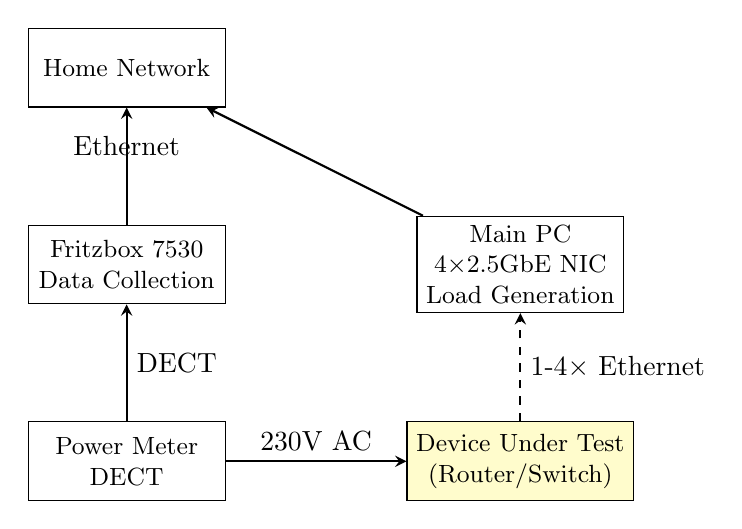
\begin{tikzpicture}[
            box/.style={rectangle, draw, minimum width=2.5cm, minimum height=1cm, text centered, font=\small, align=center},
            arrow/.style={->, >=stealth, thick}
        ]
            % Power Meter
            \node[box] (meter) at (0,0) {Power Meter\\DECT};
            
            % Fritzbox
            \node[box] (fritzbox) at (0,2.5) {Fritzbox 7530\\Data Collection};
            
            % Device Under Test
            \node[box, fill=yellow!20] (dut) at (5,0) {Device Under Test\\(Router/Switch)};
            
            % Main PC
            \node[box] (pc) at (5,2.5) {Main PC\\4$\times$2.5GbE NIC\\Load Generation};
            
            % Home Network
            \node[box] (network) at (0,5) {Home Network};
            
            % Connections
            \draw[arrow] (meter) -- node[right] {DECT} (fritzbox);
            \draw[arrow] (fritzbox) -- node[above] {Ethernet} (network);
            \draw[arrow] (meter) -- node[above] {230V AC} (dut);
            \draw[arrow, dashed] (dut) -- node[right] {1-4$\times$ Ethernet} (pc);
            \draw[arrow] (pc) -- (network);
            
        \end{tikzpicture}
        \caption{Test Setup for Ethernet Port and Speed Analysis}
        \label{fig:test_setup_rq1}
    \end{figure}

    \textbf{Test Procedure:}
    \begin{enumerate}
        \item Connect the device under test to the power meter
        \item Connect 1, 2, 3, and 4 Ethernet cables from the main PC's NIC to the device under test
        \item For each cable count, test with:
        \begin{itemize}
            \item Idle load (no traffic)
            \item 50\% load using iperf3
            \item 100\% load using iperf3
        \end{itemize}
        \item Force connections to 100 Mbps and repeat tests
        \item Force connections to 1 Gbps and repeat tests
        \item Record power consumption data via Fritzbox TR064 API
    \end{enumerate}

    \subsection{How does power consumption scale with network load (idle, 50\%, 100\% utilization of bandwidth)?}
    \label{sec:test-setup-rq2}

    \subsubsection{Test Setup}
    \begin{figure}[H]
        \centering
        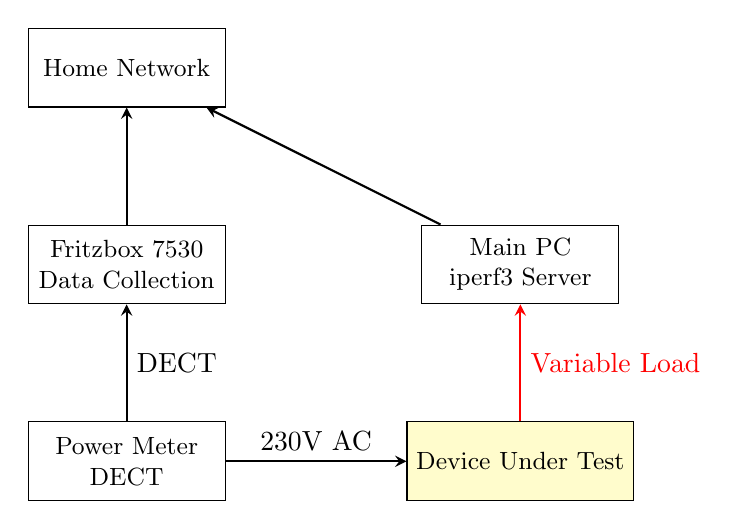
\begin{tikzpicture}[
            box/.style={rectangle, draw, minimum width=2.5cm, minimum height=1cm, text centered, font=\small, align=center},
            arrow/.style={->, >=stealth, thick}
        ]
            \node[box] (meter) at (0,0) {Power Meter\\DECT};
            \node[box] (fritzbox) at (0,2.5) {Fritzbox 7530\\Data Collection};
            \node[box, fill=yellow!20] (dut) at (5,0) {Device Under Test};
            \node[box] (pc) at (5,2.5) {Main PC\\iperf3 Server};
            \node[box] (network) at (0,5) {Home Network};
            
            \draw[arrow] (meter) -- node[right] {DECT} (fritzbox);
            \draw[arrow] (fritzbox) -- (network);
            \draw[arrow] (meter) -- node[above] {230V AC} (dut);
            \draw[arrow, thick, red] (dut) -- node[right] {Variable Load} (pc);
            \draw[arrow] (pc) -- (network);
        \end{tikzpicture}
        \caption{Test Setup for Network Load Scaling Analysis}
        \label{fig:test_setup_rq2}
    \end{figure}

    \textbf{Test Procedure:}
    \begin{enumerate}
        \item Configure iperf3 server on main PC
        \item For each device under test:
        \begin{itemize}
            \item Measure idle power consumption (5 minutes)
            \item Run iperf3 at 50\% bandwidth limit (10 minutes)
            \item Run iperf3 at 100\% bandwidth (10 minutes)
        \end{itemize}
        \item Test devices: Fritzbox 7530, Asus RT-AX68U, Alcatel HH40V, Huawei EG8245W5-8T
    \end{enumerate}

    \subsection{Which equipment is suitable for continuous operation and which devices have high idle consumption that makes them candidates for automated shutdown during off-peak hours?}
    \label{sec:test-setup-rq3}

    \subsubsection{Test Setup}
    This research question uses the same physical setup as RQ2, but focuses on long-term idle measurements.

    \textbf{Test Procedure:}
    \begin{enumerate}
        \item Measure 24-hour idle power consumption for each device
        \item Record power consumption during typical usage patterns
        \item Calculate daily energy cost at current electricity rates
        \item Identify devices with standby power $>$ 2W as shutdown candidates
    \end{enumerate}

    \subsection{How does power consumption per client differ between Ethernet and Wi-Fi connections?}
    \label{sec:test-setup-rq4}

    \subsubsection{Test Setup}
    \begin{figure}[H]
        \centering
        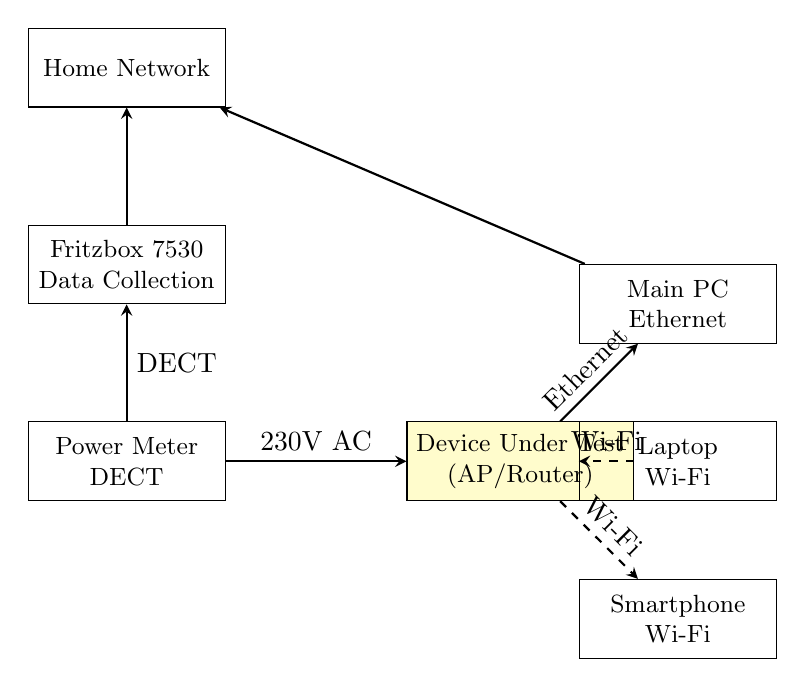
\begin{tikzpicture}[
            box/.style={rectangle, draw, minimum width=2.5cm, minimum height=1cm, text centered, font=\small, align=center},
            arrow/.style={->, >=stealth, thick}
        ]
            \node[box] (meter) at (0,0) {Power Meter\\DECT};
            \node[box] (fritzbox) at (0,2.5) {Fritzbox 7530\\Data Collection};
            \node[box, fill=yellow!20] (dut) at (5,0) {Device Under Test\\(AP/Router)};
            \node[box] (pc1) at (7,2) {Main PC\\Ethernet};
            \node[box] (pc2) at (7,0) {Laptop\\Wi-Fi};
            \node[box] (phone) at (7,-2) {Smartphone\\Wi-Fi};
            \node[box] (network) at (0,5) {Home Network};
            
            \draw[arrow] (meter) -- node[right] {DECT} (fritzbox);
            \draw[arrow] (fritzbox) -- (network);
            \draw[arrow] (meter) -- node[above] {230V AC} (dut);
            \draw[arrow] (dut) -- node[above,sloped] {Ethernet} (pc1);
            \draw[arrow, dashed] (dut) -- node[above,sloped] {Wi-Fi} (pc2);
            \draw[arrow, dashed] (dut) -- node[above,sloped] {Wi-Fi} (phone);
            \draw[arrow] (pc1) -- (network);
        \end{tikzpicture}
        \caption{Test Setup for Ethernet vs Wi-Fi Client Analysis}
        \label{fig:test_setup_rq4}
    \end{figure}

    \textbf{Test Procedure:}
    \begin{enumerate}
        \item Baseline: measure power with no clients connected
        \item Connect 1-4 clients via Ethernet, measure power consumption
        \item Connect 1-4 clients via Wi-Fi (2.4GHz), measure power consumption
        \item Connect 1-4 clients via Wi-Fi (5GHz), measure power consumption
        \item Generate identical network load across all scenarios using iperf3
        \item Calculate power consumption per client for each connection type
    \end{enumerate}

    \subsection{What is the actual impact of power-saving modes on overall power consumption?}
    \label{sec:test-setup-rq5}

    \subsubsection{Test Setup}
    Uses the same setup as RQ2, comparing devices with power-saving features enabled vs disabled.

    \textbf{Test Procedure:}
    \begin{enumerate}
        \item For devices with Energy Efficient Ethernet (EEE):
        \begin{itemize}
            \item Measure idle power with EEE enabled
            \item Measure idle power with EEE disabled
            \item Measure under load with EEE enabled/disabled
        \end{itemize}
        \item For devices with Wi-Fi power-saving modes:
        \begin{itemize}
            \item Test with various power-saving settings
            \item Measure impact on both device and client power consumption
        \end{itemize}
    \end{enumerate}

    \subsection{Does the type of connected device or wireless signal strength affect power consumption?}
    \label{sec:test-setup-rq6}

    \subsubsection{Test Setup}
    \begin{figure}[H]
        \centering
        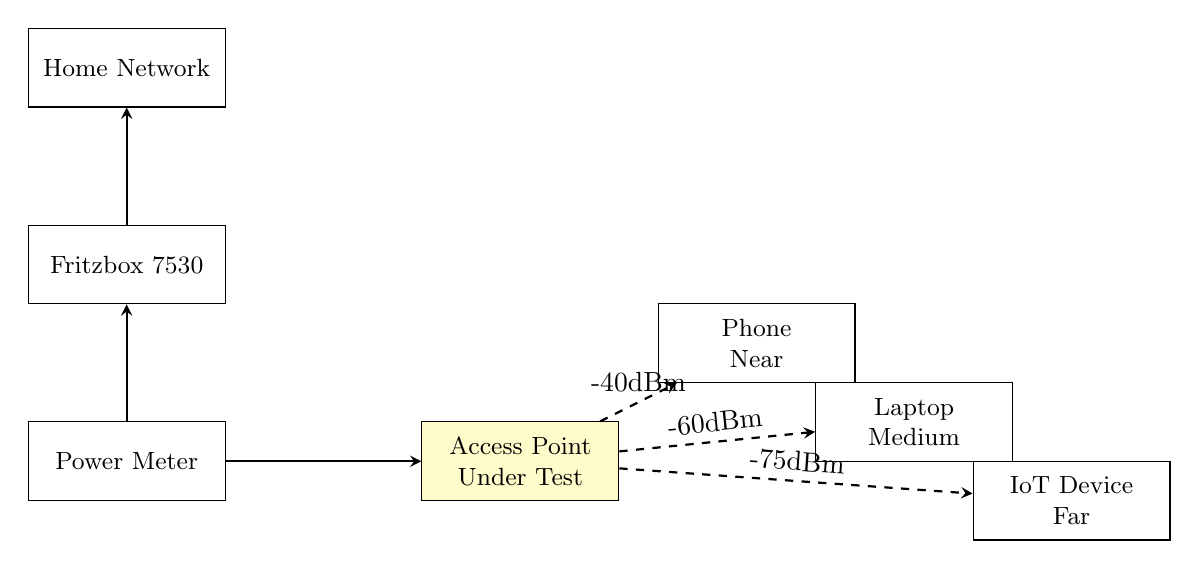
\begin{tikzpicture}[
            box/.style={rectangle, draw, minimum width=2.5cm, minimum height=1cm, text centered, font=\small, align=center},
            arrow/.style={->, >=stealth, thick}
        ]
            \node[box] (meter) at (0,0) {Power Meter};
            \node[box] (fritzbox) at (0,2.5) {Fritzbox 7530};
            \node[box, fill=yellow!20] (ap) at (5,0) {Access Point\\Under Test};
            \node[box] (d1) at (8,1.5) {Phone\\Near};
            \node[box] (d2) at (10,0.5) {Laptop\\Medium};
            \node[box] (d3) at (12,-0.5) {IoT Device\\Far};
            \node[box] (network) at (0,5) {Home Network};
            
            \draw[arrow] (meter) -- (fritzbox);
            \draw[arrow] (fritzbox) -- (network);
            \draw[arrow] (meter) -- (ap);
            \draw[arrow, dashed] (ap) -- node[above] {-40dBm} (d1);
            \draw[arrow, dashed] (ap) -- node[above,sloped] {-60dBm} (d2);
            \draw[arrow, dashed] (ap) -- node[above,sloped] {-75dBm} (d3);
        \end{tikzpicture}
        \caption{Test Setup for Device Type and Signal Strength Analysis}
        \label{fig:test_setup_rq6}
    \end{figure}

    \textbf{Test Procedure:}
    \begin{enumerate}
        \item Position clients at various distances: near ($<$2m), medium (5m), far (10m)
        \item Test with different device types: smartphone, laptop, IoT device
        \item Measure power consumption at each signal strength level
        \item Generate identical traffic patterns across all scenarios
    \end{enumerate}

    \subsection{Does maximum power rating correlate with real-world usage?}
    \label{sec:test-setup-rq7}

    \subsubsection{Test Setup}
    Uses the same physical setup as previous tests, but focuses on stress testing.

    \textbf{Test Procedure:}
    \begin{enumerate}
        \item Record rated maximum power from device specifications
        \item Measure power under maximum stress:
        \begin{itemize}
            \item All ports active at maximum speed
            \item Maximum Wi-Fi clients connected
            \item Maximum throughput on all interfaces simultaneously
        \end{itemize}
        \item Compare measured peak power to rated maximum
        \item Determine realistic power budget requirements
    \end{enumerate}

    \subsection{How efficient is ISP-provided equipment in bridge mode vs dedicated networking equipment?}
    \label{sec:test-setup-rq8}

    \subsubsection{Test Setup}
    \begin{figure}[H]
        \centering
        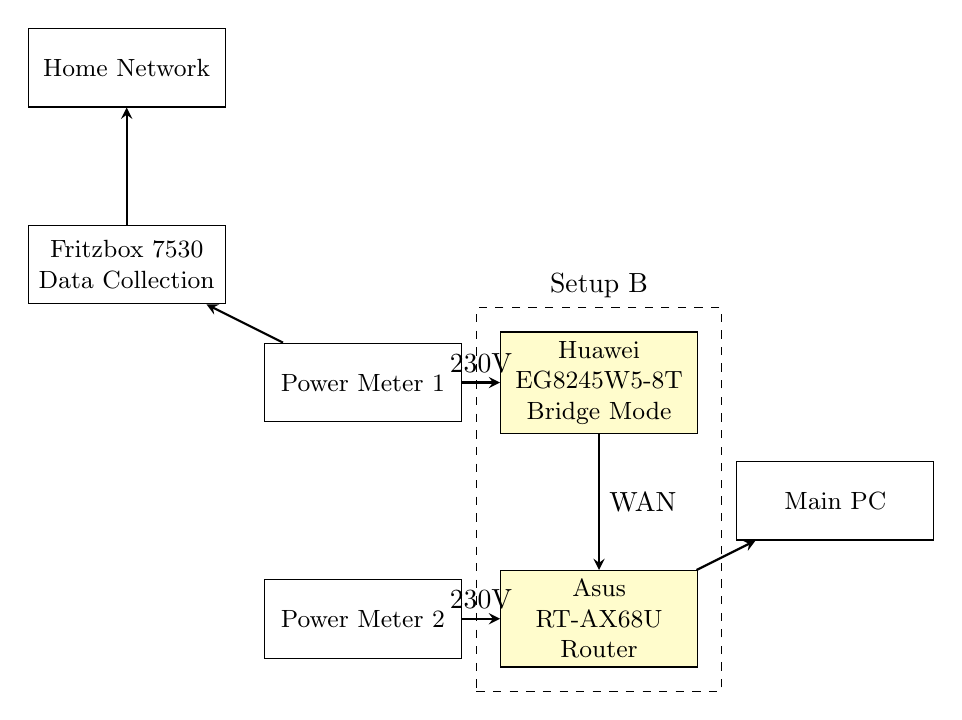
\begin{tikzpicture}[
            box/.style={rectangle, draw, minimum width=2.5cm, minimum height=1cm, text centered, font=\small, align=center},
            arrow/.style={->, >=stealth, thick}
        ]
            \node[box] (meter1) at (0,0) {Power Meter 1};
            \node[box] (meter2) at (0,-3) {Power Meter 2};
            \node[box] (fritzbox) at (-3,1.5) {Fritzbox 7530\\Data Collection};
            \node[box, fill=yellow!20] (isp) at (3,0) {Huawei\\EG8245W5-8T\\Bridge Mode};
            \node[box, fill=yellow!20] (router) at (3,-3) {Asus\\RT-AX68U\\Router};
            \node[box] (pc) at (6,-1.5) {Main PC};
            \node[box] (network) at (-3,4) {Home Network};
            
            \draw[arrow] (meter1) -- (fritzbox);
            \draw[arrow] (fritzbox) -- (network);
            \draw[arrow] (meter1) -- node[above] {230V} (isp);
            \draw[arrow] (meter2) -- node[above] {230V} (router);
            \draw[arrow] (isp) -- node[right] {WAN} (router);
            \draw[arrow] (router) -- (pc);
            
            % Alternative setup annotation
            \node[draw, dashed, fit=(isp)(router), inner sep=0.3cm, label=above:Setup B] {};
        \end{tikzpicture}
        \caption{Test Setup for ISP Equipment vs Dedicated Equipment Comparison}
        \label{fig:test_setup_rq8}
    \end{figure}

    \textbf{Test Procedure:}
    \begin{enumerate}
        \item Setup A: Huawei router in normal mode (all-in-one)
        \item Setup B: Huawei in bridge mode + Asus router
        \item Measure total power consumption of both setups
        \item Test under identical load conditions
        \item Calculate efficiency and total energy cost over 1 year
    \end{enumerate}

        %% 
%%%%%%%%%%%%%%%%%%%%%%%%%%%%%%%%%%%%%%%%%%%%%%%%%%%%%%%%%%%%%%%%%%%%%%%%%%%%%%%%

%%%%%%%%%%%%%%%%%%%%%%%%%%%%%%%%%%%%%%%%%%%%%%%%%%%%%%%%%%%%%%%%%%%%%%%%%%%%%%%%
%% 
%% Print the bibliography
%% 
%% (Optionally) let the bibliography start on a new odd page (odd is only relevant in twoside layout)
%\cleardoubleoddpage
\printbibliography
%% 
%%%%%%%%%%%%%%%%%%%%%%%%%%%%%%%%%%%%%%%%%%%%%%%%%%%%%%%%%%%%%%%%%%%%%%%%%%%%%%%%

%% Begin with the appendix part (all further sections will be appendices)
\appendix

%%%%%%%%%%%%%%%%%%%%%%%%%%%%%%%%%%%%%%%%%%%%%%%%%%%%%%%%%%%%%%%%%%%%%%%%%%%%%%%%
%% 
%% Add your appendix sections ...
%% 

%% Make sure to start the appendix on a new odd page (odd is only relevant in twoside layout)
%\cleardoubleoddpage
\section{An Appendix}
\label{app:an-appendix}

Fritzbox Web UI password: Ins2025 Wi-Fi password: default (printed on router)



%% 
%%%%%%%%%%%%%%%%%%%%%%%%%%%%%%%%%%%%%%%%%%%%%%%%%%%%%%%%%%%%%%%%%%%%%%%%%%%%%%%%

\cleardoubleoddpage

\end{document}
\endinput
